\section{Preparativos}

Antes del viaje y luego del pedaleo por Mendoza, en el primer cuatrimestre del
2005, estaba cursando en Buenos Aires el Ciclo B\'asico para Ingenier\'ia.
Despu\'es de la generosa invitaci\'on de mi viejo a visitar Europa, descripta
en la introducci\'on, empec\'e a enviar mails a mis t\'ios espa\~noles (viven
en el centro y norte de Espa\~na), a amigos (del sur espa\~nol) y a un amigo
de pap\'a que vive en el centro de Alemania, en G\"ottingen, y se llama Gustavo.
Iba a ir unas semanas, como a cualquier viaje, pero desde que empezaron los
mails comenzaban las sorpresas.

Los espa\~noles me recib\'ian con gusto, mi t\'io se tomaba vacaciones ese
verano (en Julio) para mostrarme \emph{todo} lo que quer\'ia. Y Gustavo me
contest\'o que si me quer\'ia quedar seis meses, que simplemente lo hiciera:
su casa estaba abierta; y me describ\'ia un poco (\textexclamdown \emph{muy}
poco, aunque pareciera tanto!) c\'omo ser\'ia mi vida en Alemania, queriendo
ocuparse de que no me aburriera un minuto. \'El no entend\'ia: \textexclamdown
yo curso ac\'a! \textexclamdown Estudio! De todos modos reenvi\'e ese mail a
mis viejos, para que agradecieran ellos tambi\'en la gran invitaci\'on. Los
dos contestar\'ian que era una locura, pero ver\'ian en Gustavo una hermosa
actitud.

Llegu\'e de la facultad al mediod\'ia, y me esperaban mails de ambos. El de
mam\'a me descarril\'o. Ella me iba a extra\~nar mucho, pues era una
oportunidad que no pod\'ia perder. Que lo pensara. Que irme con el ciclo
b\'asico terminado era una buena idea. Pero no cerraba ah\'i el mail porque ya
me suger\'ia en el mism\'isimo mensaje que llevara una raqueta porque a Gustavo
le gusta jugar al tenis, que disfrute de los bosques de alrededor, y de lo
amigable de la gente de su barrio. \textexclamdown Y yo esperaba recibir
solamente un ``qu\'e lindo gesto el de Gustavo''! Emocionado y todav\'ia
incr\'edulo, le\'i el de pap\'a. Avalaba lo que dec\'ia mam\'a, me autorizaba a
tomarme medio a\~no de vacaciones (\textexclamdown con tanto estr\'es lo
necesitaba!), y me daba libertad de volver cuando quisiera, sea a los 2, 3 \'o 6
meses.

Imaginen por d\'onde volar\'ia mi cabeza esos tiempos, que fui a rendir el
\'ultimo parcial con el dinero del pasaje en el pantal\'on. Le ped\'i
compa\~n\'ia a un amigo que terminaba de rendir conmigo, \'el no pod\'ia creer
que rindiera y caminara tranquilo con eso\ldots\ \textexclamdown En realidad
yo tampoco lo pod\'ia creer!

El 5 de Julio, cena despedida en casa: familia nuclear, un amigo y yo. Las
corridas de no olvidarme de nada, los documentos, la plata, llevarlo a mi
hermano a la casa, a mi amigo, dormirme, despertarme, ba\~narme, vestirme. Los
``\textquestiondown Ten\'es la billetera? \textquestiondown Y d\'onde?''
``\textquestiondown Llev\'as los documentos en un lugar seguro?
\textquestiondown D\'onde?'' Cerrar el bolso a \'ultimo momento pero
asegur\'andome de no dejar nada\ldots

El 6 a la madrugada, foto en Ezeiza y despedida con mis viejos. S\'olo los
hab\'ia visto emocionados por este viaje a trav\'es de internet, pero ahora en
persona. ``Chau''. Es tan simple que me molestaba sentirlo, pero de verdad que
no es f\'acil decir ese ``chau'' por un tiempo. Pas\'e todo ese d\'ia
sentadito, escuchando a las turbinas alej\'andome de a cientos y miles de
kil\'ometros de todo continente conocido. Pensaba en lo impresionante que era
todo. Hac\'ia horas hab\'ia rendido y ahora estaba viajando a Espa\~na, donde
me esperar\'ia una rama familiar divina y que nunca conoc\'i.

En la madrugada del 7 llegu\'e a Madrid. Busqu\'e la mochila, y a ver si me
recibe la familia y nos reconocemos\ldots

\section{Espa\~na y familia europea}

\subsection*{Jueves, 7 de Julio}

\textexclamdown Hola Familia y amigos! \textquestiondown C\'omo andan?
\textexclamdown Por aqu\'i todo bastante bien, a pesar de todo!

Me voy a olvidar del 90\% si no escribo todo porque son \emph{tantas} cosas
juntas las que aprendo y veo y admiro, que seguramente se me pasa gran parte, y
de no escribirlo se me pasar\'ia casi todo. Sin estos espa\~noles que me llevan
de la oreja para cada lado no sabr\'ia que hacer. Conocen mucho de su historia,
y pueden transmitirla con facilidad.

Empezando desde el vuelo, buen d\'ia al despegar y noche clara al aterrizar.
S\'olo nublado durante el vuelo. El poco tiempo que compart\'i con mi
compa\~nera de viaje me mor\'i de risa. Era de tu edad, Ma, y ten\'ia las
mism\'isimas peleas con el hijo que vos y yo al viajar. Antes de hablar de
eso me hac\'ia chistes como si fuera un amigo cualquiera: ve\'iamos el video
de precauciones del avi\'on y dec\'ia (entre otros) ``\textexclamdown oye
Manolo, que ha llegado el cotill\'oon!'' cuando tiraban las mascarillas de
gas. Est\'abamos tentados, \textexclamdown qu\'e buena onda que hay de viaje!
Despu\'es fue a otro asiento as\'i dorm\'iamos m\'as c\'omodos.

Reci\'en ca\'ia de lo lejos que voy al descender, viendo el mapa. Cruzamos
Brasil hasta llegar al Atl\'antico, \textexclamdown y ahora estoy en el viejo
mundo! Viejo literalmente, si hablamos de ``civilizaci\'on'' como la
entendemos.

Mi ritmo circadiano todav\'ia no capta la hora de ac\'a ni la de Argentina,
los espa\~noles se r\'ien porque de noche doy vueltas, y de d\'ia duermo
profundamente y no me pueden despertar. Dicen que duermo ``m\'as que las
s\'abanas''.\\

El primer d\'ia fuimos V\'ictor (t\'io madrile\~no), Daniel (primo asturiano)
y Eugen\'in (padre de Daniel, y responsable de mi nombre) a Segovia. Es una
ciudad famosa por conservar un acueducto del siglo segundo, formado por
piedras encastradas perfectamente. Lo sorprendente adem\'as es que se us\'o
hasta hace pocos a\~nos, cuando la falta de eficiencia lo tornaba caro
(evaporaciones fue lo \'unico que me explicaron). Funcion\'o durante 1800
a\~nos.

De ah\'i vimos la muralla de estas ciudades de \'epoca; un ``alc\'azar''
(``castillo'', para m\'i) t\'ipico de dibujitos con agua al rededor, puente
levadizo y grandes muros y torres; y muchas casitas y callejuelas antiguas.
Todo pintoresco, no se les escapa la tortuga ni en peque\~nos detalles.

A la vuelta nos pas\'o por la autopista una Ferrari 360 descapotada \emph{muy}
r\'apido. \textexclamdown Son\'o tan fuerte, pero tan poco tiempo a nuestro
lado! Dicen que si te pescan a m\'as de 180~km/h por las autopistas te quitan
el carnet por tres meses, aparte de cobrar una jugosa multa. Un ejemplo a
imitar. No v\'i autos viejos, tampoco ``baratijas'' de esas que ni {\small
ABS} traen y llegan a 140~km/h.

Al llegar a Madrid conocimos su parte vieja. A mi me re-sorprenden, pero ac\'a
deben ser moneda corriente estas antig\"uas urbanizaciones. Vi calles de dos
metros de ancho, es decir que para salir de la casa uno tiene que inclinarse
antes sobre la puerta sin bajar un pie, para asegurarse de que no pasan
veh\'iculos y se puede bajar. Las estrechas callejuelas serpentean por donde
los constructores quisieron, y hay tantas ondulaciones que un poco por
perspectiva y otro por el ceder del terreno, se ven las casas inclinadas hacia
la calle. Es decir que no se ven las paredes perpendiculares al piso,
\textexclamdown por las dudas no pisar\'ia las plantas m\'as altas!

Vimos por {\small TV} las corridas t\'ipicas de Pamplona, esas que largan
toros por la ciudad hasta la plaza mayor, y la joda dura una semana seguida.
\textexclamdown Hay mucho que aprender de estas culturas tan avanzadas!\\

La segunda ma\~nana (siento que son m\'as por todo lo que recorrimos) sal\'i a
correr temprano por ``el Retiro'', el equivalente a Palermo de Madrid. Se
diferencia por ser m\'as ``parque'' y menos ``salvaje'', y por estar no
alejado sino en \emph{medio} del centro de la ciudad. Corr\'i poco y
sufrido, entre el verano y poco entrenamiento. % Conflicto de días?

Luego del desayuno, fuimos con Eugenio a Toledo. Conoc\'i la catedral, es
\emph{inmensa} y llena de capillas adentro; no podr\'ia juzgar cu\'al es m\'as
impresionante. Son tantas cosas por metro cuadrado que no tengo dudas de que me
perd\'i la mitad, y me llev\'e la otra mitad. De todos modos si quer\'ia ver
todo seguro terminaba cansado y sin ganas de ver un s\'olo Cristo m\'as. Es, muy
resumidamente, una enormidad que emana arte por donde miren. Por dar un ejemplo,
los coros se sientan en sillas tipo teatro: al levantarse, sube donde apoyan las
sentaderas. Pero es de madera vieja, oscura y fuerte, y tiene trabajos tallados
abajo del asiento para que cuando no est\'an ocupadas se vean. Y son muchas,
pero no hay dos motivos repetidos. No hay simetr\'ia de im\'agenes. Demasiado
lujoso con trabajos en todos los rincones. Desde la primera piedra al \'ultimo
detalle corrieron 300 a\~nos de desarrollo. Deber\'ian ver las cerraduras de la
\'epoca. En medio de las pesadas puertas de madera, impresionan por el tama\~no.
Las argollas son de 8cm de di\'ametro y guardan a esas llavezotas del tama\~no
de un martillo.

Volvimos, profunda siesta, profundo almuerzo (almorzamos siempre buena comida,
gracias al cocinero de lujo que es V\'ictor), y salimos para el Palacio real.

Son cientos de habitaciones, y en cada una hay que ver paredes, techo y suelo
para empezar; para luego observar todas las sillas, muebles, pinturas, figuras,
vajillas, etc. Paredes cubiertas con tapices tejidos a mano de diferentes
colores y estilos (todo de lo m\'as perfecto y de cualquier lugar del mundo),
techos con frescos y adornos en oro que hac\'ian de marco, adem\'as de
ornamentales ara\~nas por todos lados (que, dicho sea de paso, ten\'ian las
bombitas de luz trabajadas); pisos con diversos tipos de m\'armoles, cortados
perfectamente para que al encastrarlos formen figuras; mesa para 144 comensales
donde cada silla debe valer como\ldots\ un viaje a Disney. \textexclamdown
Pasillos revestidos de invalorable arte, y no son m\'as que pasillos! Un
empalago de lujo. Luego, a la armer\'ia, donde hab\'ia maniqu\'ies de caballeros
medievales, con sus caballos protegidos por armaduras tambi\'en. Varios modelos
de este elegant\'isimo deporte (creo que se llamaban ``juntas''), me
encantaron. Las espadas est\'an todas buenas y curiosamente no pasan los
\geneuronarrow{70}. Trabajadas, grandes, pesadas\ldots\ \textexclamdown Ver\'an
que perd\'i la tabla de conversi\'on al peso! Sino no puedo juzgar qu\'e es caro
o barato, porque todo es caro, o caris\'isimo.

Ma\~nana me castigar\'an con el Escorial y el Valle de los Ca\'idos. Estar
ac\'a, con \emph{toda} esa historia que cuentan, y as\'i entender el porqu\'e
de cada detalle (no solo el hecho de ver las fara\'onicas construcciones),
conmueve. Esa tarde llegar\'e a Gij\'on, Asturias, para luego recorrer toda la
zona Norte que promete ser interesante, adem\'as de m\'as verde. Y conocer\'e
a Carmen y Jorge, esposa e hijo menor de Eugen\'in. Hoy desped\'i a Daniel que
se va de viaje, le agradec\'i la compa\~n\'ia y buena onda.

Les cuento que Mar\'ia, mujer de V\'ictor, me cag\'o a pedos por usar los dos
d\'ias la misma remera, y me la exigi\'o para lavar. \textexclamdown No se
qu\'e problema se hac\'ia, si al llegar de vuelta a Pergamino la iba a lavar
yo!\\

PD1: Ac\'a son ``rar\'isimos'' los enchufes planos de patas oblicuas, menos
mal que consiguieron un buen adaptador por ah\'i.

PD2: Saqu\'e la billetera s\'olo para comprar ese adaptador\ldots\
\textquestiondown atentos estos espa\~noles?

\subsection*{S\'abado 9 de Julio}

\textexclamdown Hola! Muchas gracias por sus mails, si bien parecen fr\'ias
las {\small PC}s deben ser otra causa que ``aiuda'' a que no extra\~ne un
``co\~no''.

El s\'abado Uge me levant\'o (dos veces, como siempre) para desayunar y salir.
Dorm\'i como nutria, as\'i que estuve bastante despierto. Desped\'i a V\'ictor
y familia, por ah\'i los vuelva a ver por Cand\'as. Visitar\'an a la madre de
Eugenio luego de una operaci\'on. \textexclamdown Es incre\'ible esa mujer! Ya
llegar\'e.

Salimos en el auto y, como siempre, no ten\'ia idea a donde me llevaban pero
el paisaje me encantaba. Dicen que hay muchos accidentes de tr\'ansito a pesar
del gran orden. Cuando coment\'e mi sorpresa por el orden, respondi\'o
V\'ictor: ``Vas a ver lo que es el orden cuando conozcas Alemania'', y todos
concordaron. \textexclamdown Qu\'e diferente ser\'a, para que estos
espa\~noles declaren su tr\'ansito desordenado!

Paramos en un lugar por fuera bastante simple (en relaci\'on a Espa\~na,
porque si lo veo en Pergamino me siento al lado para mirarlo como a glaciares),
despu\'es supe: El Escorial. La visita fue interesant\'isima. El rey Felipe
II era humilde (tambi\'en en relaci\'on a otros reyes, porque esta enormidad
era su casa de veraneo) y construy\'o de granito (piedra com\'un) todo su
castillo. Pinturas por todos lados, solo me impresion\'o de verdad algunas
aberturas (trabajos de minuciosa marqueter\'ia: miles de maderitas de distinto
tipo pegadas unas junto a otras, que forman im\'agenes y dan sensaci\'on de
profundidad). Tambi\'en me llen\'o la vista desde las ventanas, a un precioso
jard\'in todo ornamental, a la enormidad de un muro del palacio --que la
perspectiva acusaba su tama\~no--, a las verdes sierras; y, m\'as al fondo, al
lejano y bajo suelo, amarillo por el trigo. Luego bajamos al pante\'on de la
realeza.

Felipe quiso simpleza e hizo todo de granito, pero los hijos dijeron:
``\emph{\textexclamdown puez co\~no, que ezte hombre mereze m\'az
imponenzia!}'' (aunque no es descabellado que fuera para ellos), y cubrieron
de m\'armoles azules y rojizos \emph{toda} la larga escalera que baja y el
pante\'on; y lo iluminaron con ara\~nas de oro. En el recinto, si no se ve
m\'armol es por los adornos de oro que los tapan. Nos explicaron el orden en
que los van enterrando, y qu\'e har\'ian cuando se acaben los lugares (quedan
tres).

Subimos al pante\'on de los infantes, con capacidad para m\'as de cien. El
impresionante lujo de este pante\'on qued\'o opacado por el anterior. Lo que
m\'as me movi\'o fue la cantidad de ni\~nos enterrados, no s\'olo por la no muy
avanzada medicina de la \'epoca, sino tambi\'en por los problemas con que nacen
los hijos de familiares cercanos; y aqu\'i arreglaban as\'i los casamientos.

Como los cajones son peque\~nos para un cuerpo, los difuntos esperan 30 a\~nos
en el ``pudridero'', para poder ser luego reducidos y alojados en sus
respectivos cajones. Los ``pudrideros'' (nombre muy figurativo, ya lo dijo la
gu\'ia) est\'an a los costados de la escalera entre-panteones.

Era clara la importancia de la iglesia en la \'epoca: es lo m\'as lujoso de
todo el castillo. En esta casa de retiro espiritual para Felipe tambi\'en
funcionar\'ia un monasterio. Iglesia enorme, con miles de detalles de los que
cualquier conocedor de arte se maravillar\'ia, y con los dormitorios a los
costados del gran altar. As\'i, Felipe, (que vivi\'o mucho para su \'epoca, y
pasaba gran parte de sus \'ultimos tiempos en cama) pod\'ia seguir la
celebraci\'on.

Visitamos luego la incre\'ible biblioteca, tambi\'en m\'as lujosa que el
propio palacio, con varias particularidades. Cientos de libros guardados al
rev\'es (las hojas hacia afuera) para que la humedad no los arruine. Los
t\'itulos son escritos sobre las hojas, previamente ba\~nadas en oro. Algunos
son inmensos, con oro en cada hoja y un trabajo que por cada letra yo
invertir\'ia horas. Las mesas de m\'armol sosten\'ian antiguos globos
terr\'aqueos, es interesante pensar en c\'omo diagramar\'ian el mundo con
herramientas tan precarias y viajes tan largos. Hab\'ia un globo con la tierra
en el centro y varios anillos circulares al rededor, que ilustraban el
movimiento de estrellas, sat\'elites y planetas, mostrando a la Tierra como
centro del Universo. V\'i la foto de esta biblioteca en alg\'un libro de la
secundaria, l\'astima que no estudiamos suficiente (obvio, \textexclamdown
porque no estoy ah\'i en el pupitre lo pienso!)

De ah\'i, a un largo pasillo con im\'agenes de guerra y batallas en las
paredes, y ventanas intercaladas. Si ven las guerras de la \'epoca salen
corriendo antes de que disparen la primera lanza. Es sorprendente, me dieron
ganas de ver pelis de la \'epoca. \textexclamdown Y hasta de leer! A la salida
nos esperaba un pasillo donde mostraban c\'omo fue construido todo, mediante
maquetas e im\'agenes. Las gr\'uas, poleas, diagramas\ldots\ es
\emph{indescriptible}. Linda civilizaci\'on.

Salimos al pueblo, y conoc\'i una sinagoga, sorprendente por su bella
simpleza; varios comercios de cosas t\'ipicas, im\'agenes de Don Quijote
(soldado por excelencia, seg\'un me cuentan) y otras yerbas. Buena vista,
entre el palacio sobre una sierra y la planicie madrile\~na.\\

Despu\'es visitar\'iamos el Valle de los Ca\'idos, la humilde tumba de Francisco
Franco cavada dentro de una cueva de piedra, constru\'ida por cientos de presos
pol\'iticos. De esto esperaba \emph{tanto}, que recib\'i lo que esperaba. Ya
conoc\'ia por fotos y descripciones. No pude dejar de pensar en la actualidad de
las ideas (actuales, de hecho), y de c\'omo fue construido, as\'i que esto me
impresion\'o desde el lado hist\'orico, humano. \textquestiondown Bello? Obvio,
pero al esperarlo lo disfrut\'e sin impresionarme como con todo. S\'olo
captur\'e a esas esculturas de un l\'ugubre monje que escoltan los h\'umedos
pasillos, escalofriante. Cercaron la tumba de Franco con una bonita soga para
que no la pisen, la miraba atento mientras Uge insist\'ia en que levante la
vista para poder ver un mosaico en el techo que mostraba, como en todos los
lugares que visitamos, im\'agenes religiosas, casi siempre cat\'olicas. Antes de
entrar le preguntaba a Uge si a los espa\~noles les perturba visitar un
monumento a la tiran\'ia (de modo m\'as suave y menos ``Lisa Simpson''), y me
contest\'o que le ``importa un coj\'on''. Todav\'ia me estoy riendo y
memorizando la frase.

No pude apreciar la inmensidad de la cruz de arriba por no poder acercarme,
pero se supone por lo grande que se ve si bien est\'a tan alta, y al alejarse
se sigue distinguiendo f\'acilmente. Al llegar a Gij\'on, Jorge (su hijo) me
daba m\'as argumentos por los que toda guerra es irracional y fundada en odios
que ni siquiera existen en el momento: su bisabuelo ni sab\'ia si era
republicano o del otro bando, y sin embargo, en su ignorancia de simple
pescador, qued\'o encerrado en una vieja iglesia. El ir a la iglesia o no era
raz\'on suficiente para pertenecer a uno u otro bando. Divisi\'on binaria por
excelencia.\\

\textexclamdown Veo las fotos para no olvidarme, y entiendo lo movido que
estuvo el d\'ia! En viaje a Gij\'on paramos en \'Avila, que mostraba un muro y
torres pero de lo m\'as t\'ipico que podamos imaginar, y de las m\'as
antiguas. Oscuras, largos muros interrumpidos por altas torres con almenas.
Excelent\'isima vista desde all\'a arriba. Almorzamos en un restaurant de lujo
con un poco de sue\~no. Luego, la vista de la ruta a Gij\'on no me permitir\'ia
dormir.

En viaje vi parques e\'olicos y peque\~nas pantallas solares. Hay puentes
tapados por madera que cruzan la autopista de campo abierto a campo abierto
(no une caminos) para que los animales salvajes sigan su curso, y que la nueva
autopista no rompa el equilibrio de la regi\'on. Esto es demasiado. Cuentan
que una obra se retras\'o varios d\'ias para esperar a que nacieran unos
halcones en peligro de extinci\'on. \textexclamdown A cada minuto corresponde
un comentario! Hay cig\"ue\~nas en cada lugar alto, hacen unos nidos enormes.

Cruzamos el t\'unel a Asturias. Lo bueno, adem\'as del camino sinuoso y
serpenteante entre verde y boscoso, con subidas y bajadas, es que a Uge le
gusta manejar, y lo hace bien. Nunca pas\'o los 140~km/h con control de
velocidad crucero (o casi). \textexclamdown Pero en curvas tampoco los baj\'o!
No conoc\'ia la marca Honda, si es para viajar en rutas es un placer.

Llegamos al atardecer del viaje de Madrid. Me acomod\'e, cen\'e, y sal\'i
hasta las 3 am (muy buena onda los amigos de Jorge). Hoy a la ma\~nana salimos
a correr por la costanera, al sol y en remera. \textexclamdown En Julio! Por
este camino hay varias obras de arte moderno y abstracto, desentonan con el
clasicismo al que vengo acostumbrado. (En mi vida cre\'i que hablar\'ia de
arte.)

Hoy almorc\'e en lo de la madre de Uge, Josefa, en Cand\'as; cocin\'o la
sobrina Lily y es tambi\'en cocinera de lujo. No paro de comer, pero no
entiendo porqu\'e ac\'a lo hago lento si en mis 19 a\~nos nunca lo hice. Vimos
la F1, ac\'a se mean por Alonso como all\'a por todos los corredores del
{\small TC} juntos. Va bien en el campeonato. Visita tur\'istica a este pueblo
ma\~nana, pues hoy internaban a Josefa. Esta mujer no se puede creer: es la
delicadeza de una abuela con el humor m\'as\ldots\ \ \textexclamdown o menos
de abuela!, que se puedan imaginar. Me re\'i m\'as que con Uge. Jorge se
hab\'ia olvidado unas pastillas en la casa, y entonces le dijo: ``Pero queriido,
\textquestiondown ninguna de las m\'ias le va?'' Sonriendo p\'icara.
Incre\'ible, qu\'e hermosa actitud hacia la vida.

Me interrumpieron la escritura (no es raro si estoy ac\'a hace tiempo) para
presentarme a dos t\'ias de Jorge. Divinas, una es Ingeniero Qu\'imica
apasionada, capa en energ\'ia at\'omica (me explica que toda casa que se
edifique en Espa\~na debe tener paneles solares, de manera de no depender
100\% de un \'unico sistema energ\'etico). Charlamos un mont\'on,
interesante. Y as\'i termina el Domingo, ahora a dormir ``m\'as que las
s\'abanas'' para ma\~nana visitar Cand\'as.\\

PD1: \textquestiondown Vieron qu\'e palabra, ``pupitre''?

PD2: \textexclamdown Co\~no, que ze me ezt\'an pegando algunaz palabraz
ezpa\~nolaz!

PD3: Existi\'o un s\'olo ``gallego'' como los conocemos o prejuzgamos, y fue
quien invent\'o el bidet. \textexclamdown Todav\'ia no s\'e usarlos!

\subsection*{Lunes 11 de Julio}

\textexclamdown Me olvid\'e de describir el Parlamento donde sesionan en
Madrid! Fue incre\'ible: pasamos tres filtros hasta lograr entrar (no cerraron
el auto, por ejemplo, por los sensores de infrarrojos que hay al rededor).
Est\'an en obras y dirige V\'ictor, por eso pudimos pasar. Aparte de la
cantidad de sillas bonitas, tanto arte, lujo, y la silla del rey, lo que m\'as
me impresion\'o fue 4 agujeros de bala que dejaron en 1981 durante un intento
de golpe de estado. Estuvieron unas horas con tanques en la calle, pero las
fuerzas armadas en general no les dieron bolilla seg\'un me cuentan.

Caminamos todo Cand\'as, para ver las cosas que ya esperaba; si bien
\emph{todo} es bello, nada me sorprendi\'o. Vi desde un camino alto la casa de
nuestros bisabuelos, conoc\'i el ``Cristo con falda'', desolador, en una
incre\'ible capilla; dimos una vuelta por una pen\'insula alta, donde adem\'as
de toda la vista al Mar Cant\'abrico encontramos una capilla al santo de los
novios creo, hermos\'isima, simple y chiquita, y armada as\'i nom\'as en lo
alto del monte. Bajamos al puerto y vimos el faro a le\~na, la pe\~na furada
(una gran piedra en la playa agujereada al medio, a veces tapada por el agua y a
veces sobre la seca arena debido a las contundentes mareas diarias), y tom\'e
agua de una fuente que hace a quien la bebe ``despierto, atento''. Esperan
desde ahora no trabajar tanto al despertarme. \textexclamdown Me parece, ahora
que lo pienso, que me trajeron a Cand\'as s\'olo para esto! Muchos detalles en
este bonito e hist\'orico pueblo.

Despu\'es, lo mismo por Gij\'on. Recorr\'i bastante, conoc\'i mucho, caminamos
por su parte antig\"ua, tomamos sidra tirada (desde la botella, vertiendo desde
el brazo estirado por sobre la cabeza, hasta el vaso, que espera el l\'iquido a
la altura de la cintura), que estaba bastante buena pero no es de mi devoci\'on
(tiene buen gusto a jugo de manzana). \textexclamdown Y me empec\'e a re\'ir con
las puteadas del gallego! \textexclamdown Hab\'ia tanto viento que enchastraba
todo menos el vaso! \textexclamdown Se daba vuelta como mirando al viento para
putearlo! Muy gracioso.

Al otro d\'ia salimos de Gij\'on para conocer la Universidad Laboral.
Imponente, pregunt\'e la ``\'epoca'' en que fue constru\'ida, y tiene s\'olo
alrededor de 60 a\~nos. Franco mand\'o a construirla como orfanato minero,
pero nunca se lleg\'o a usar para eso, y ahora funciona como escuela y
universidad. Es del estilo de los alc\'azares, no la describir\'e en detalle
pero daba esa imagen. Mil cosas incre\'ibles (que la alumna de secundaria,
voluntaria en vacaciones, nos relataba al guiarnos) y una que me interes\'o
m\'as que todas: al sacar los andamios de la capilla con forma ovalada el
techo cedi\'o 30 cm, y por eso la cruz que est\'a grabada en la punta ya no
proyecta la luz del sol camino al altar. La universidad est\'a bastante alta,
y subimos a su torre de 17 pisos para apreciar Gij\'on. Una maqueta.

De ah\'i a un hermos\'isimo gran parque en la otra pen\'insula Este de Gij\'on,
no la que ya recorrimos. Hab\'ia una edificaci\'on chica tipo trinchera que se
us\'o durante la guerra civil. No se el nombre: t\'ipico ver dos soldaditos
metrallando ah\'i encerrados, y un enemigo que les mete una granada adentro, eso
era (``b\'unker''). Muy impresionante verlo ahora, todo libre y
desmilitarizado. Se cerr\'o su entrada, no por las granadas sino por las
bombitas de olor que dejaban algunos borrachines. Un pesquero y dos yates nos
indicaban d\'onde estaba el mar, que se confund\'ia con el cielo.

\begin{center} 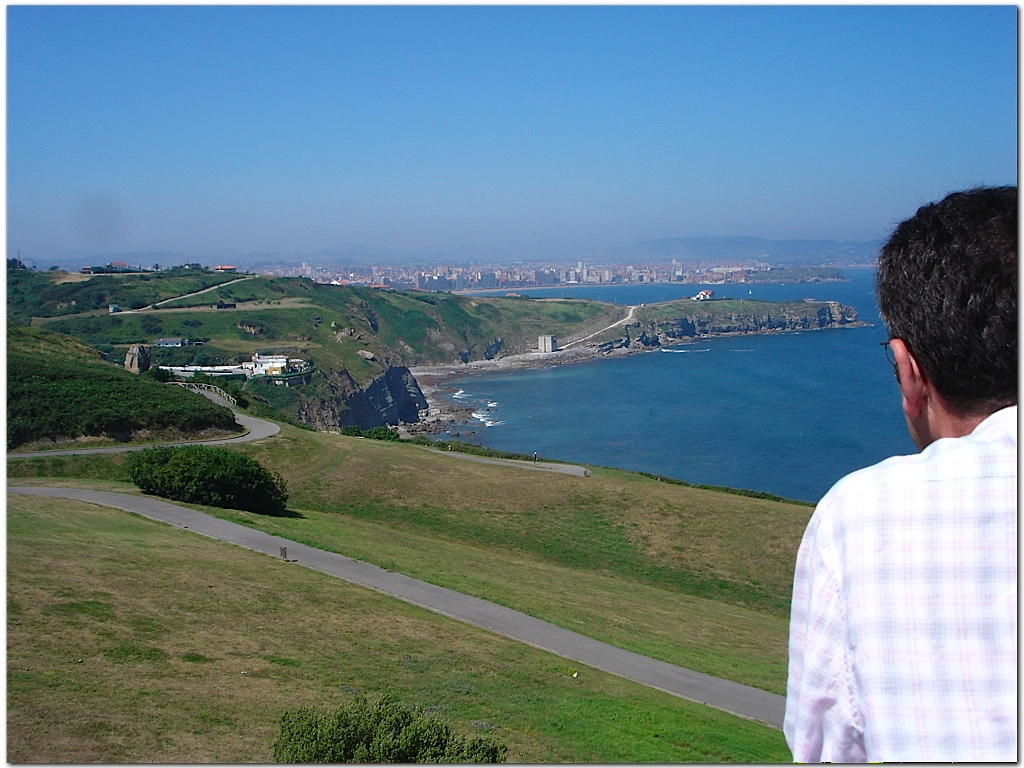
\includegraphics[width=300px]{images/Espana-805.JPG}\\
\textsc{Mirador Este de Gij\'on.} \end{center}

Bajando un poco por la costanera una escultura: ``la madre del emigrante''. Es
la primer escultura que me conmueve, lo llena a uno de esa desolaci\'on que el
artista habr\'a querido imprimir. Ver de este lado lo que estudiamos all\'a
como ``inmigraci\'on'' es simplemente esa imagen.

Esa tarde me met\'i en el mar. Terriblemente fr\'io al entrar, muy relajador
al salir. Y estar, un placer, desde que uno se acostumbra a las algas. Azul,
con pocas y suaves olas, y sin bancos de arena ni pozos, no tiraba ni para el
costado. Lo m\'as destacable es que en la escalera 7 (hay varias y bastante
unidas) estaba prohibido ba\~narse, y yo estaba en la 5. Las mareas y
correntadas cambian en pocos metros. El estar reci\'en llegado todav\'ia me
hac\'ia sentir el placer de meterme al mar en ``invierno''.

\begin{center}
  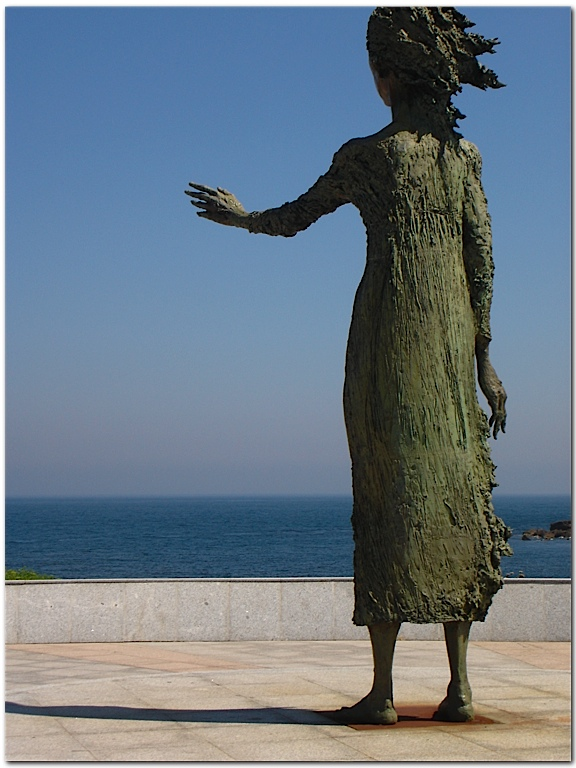
\includegraphics[width=200px]{images/Espana-812.JPG}\\
  \textsc{La madre del emigrante.}
\end{center}

En la tarde, la frutilla del postre: Covadonga. Un camino a los lagos que Uge
no recorr\'ia desde hac\'ia 30 a\~nos. Es \emph{perfecta} esa ruta, me dieron
ganas de comprarme una bici y recorrerla toda, y volver a Gij\'on por caminos
de tierra. De esos paisajes que se ven en postales suizas o austr\'iacas se
trata. Los terrenos, muy chicos, est\'an divididos por arbustos. Lo t\'ipico
de las postales de aqu\'i: una gran catedral con la imagen de la Virgen de
Covadonga, y un excelent\'isimo sagrario (en realidad lo repelo bastante, muy
tur\'istico y comercial me pareci\'o). Lo lindo de la catedral era verla inmersa
ah\'i, en ese bosque tan divino. Arriba de una sierra hay una imagen de Pelayo y
la cruz, donde seg\'un la leyenda ``casi'' se cae, y un camino que la un\'ia a
donde est\'abamos. \textexclamdown Me dieron buenas ganas de subir! Pero era
largo dice Uge. Despu\'es, la cueva donde apareci\'o la Virgen, hermosa la
imagen y la vista. Pero de nuevo lo mismo, yo estaba mala onda me parece por la
cantidad de cosas que se vend\'ia, y de gente curiosa como yo. Y de ah\'i, al
para\'iso.

Una ruta casi de una mano subiendo sin parar, escoltada por mucha vegetaci\'on
\emph{verde}, a veces tipo t\'unel; algunos ciclistas subiendo (en pocas horas
ser\'ian los m\'as felices del mundo con la cantidad de curvas que hay),
vaquitas en medio de la ruta con cencerros, y algunas ovejas de pelaje largo.
Primer mirador: desde muy alto a los valles verdes, a la ahora lejana catedral,
y atr\'as, los picos nevados. \textexclamdown Nieve! La ruta se ve\'ia por
cualquier ventanilla del auto serpenteando a trav\'es del bosque. Seguimos hasta
encontrar un auto parado: el conductor intentaba espantar a las vacas sueltas.
Miles que est\'an buscando sombra caminan por estas monta\~nas, parte de los
``Picos de Europa''. Salimos temprano para no encontrar demasiada gente, y dio
resultado.

Primer lago, y tras un cerro el segundo lago. Paramos, caminamos hasta el
cerro y se pod\'ia ver los dos lagos, adem\'as de diversos caminos para seguir
a pie. Paradis\'iaco.

Bajamos y cruzamos los tradicionales horrios, construcciones de madera
levantadas del suelo para guarecer a las vacas del sol, y guardar granos
alejado de las ratas. Conoc\'i el puente de Covadonga, lo conozco de
memoria por fotos y, a diferencia de lo que cre\'ia, est\'a en una ciudad;
pero verlo ``en serio'' fue maravilloso. Es como todos los castillos, uno sabe
que son as\'i, pero estar se siente diferente. Esta zona me enamor\'o.

Volvimos por la ruta ``vieja'' para parar en un museo de sidra (interesante,
lo m\'as: las prensas que usaban hace doscientos a\~nos, de madera y con
palancas, a m\'as larga mejor); y para disfrutar de las incontables curvas, que
si uno se cerraba demasiado choca con la sierra, y si se abre, contra el
guarda riel. Y Uge maneja muy bien as\'i que no se nos dificult\'o disfrutar
de esto \'ultimo. Vimos Gij\'on desde el d\'ecimo mirador (a cu\'al m\'as
hermoso), y vuelta a casa.

Me preguntan qu\'e como, y como como como en casa (\textexclamdown qu\'e
trabalenguas!) S\'olo que usan otras especias, pero todo muy producido y rico.
Nunca de m\'as ni tampoco de menos, bien medido. Si estaba rico y somos
glotones, \textexclamdown s\'olo entonces nos quedamos cortos! Pero
relativamente. Buena costumbre a la que no acostumbramos.

Y ahora ver\'e si el calor me permite correr como espero. Sino, al mar.
\textexclamdown Hay tantos problemas por los que preocuparse, en esta zona! Lo
comparaba con el viaje de 5$^\circ$ a\~no en ese sentido. Fuera de broma, hoy es
tapa del diario la sombra de un tibur\'on que apareci\'o en las playas, pero
dicen que no hace nada. Ya les contar\'e. O tal vez no\ldots En fin,
\textexclamdown de cualquier modo, saldr\'e a conocer!

\subsection*{Mi\'ercoles 13 de Julio}

Es impresionante c\'omo escribo pensando que pasaron varios d\'ias, pero son a
lo sumo dos.

La tarde despu\'es de Covadonga sal\'i a correr por la costanera hasta el
mirador del Este, que me hab\'ia encantado. Hab\'ia ido en auto y me enga\~n\'o:
la costanera est\'a \emph{llena} de subidas y bajadas. Pensaba ir y volver sin
parar pero, fulminado, me tir\'e en el mirador a contemplar las maravillas de
este infierno. Estaba ventoso. Volv\'i trotando, me tir\'e en el mar vestido
como estaba, y, ya en casa, me d\'i una \emph{gran} ducha. Luego una siesta de
20 a 22hs antes de cenar (fulminado, en serio), \textexclamdown y a la Semana
Negra!

La Semana Negra es una gran feria anual en Gij\'on, que tiene cosas tan variadas
e inconexas que da risa el s\'olo mirar. Los puestos son tipo la Rural de
Pergamino, pero el tema, nada que ver. Empez\'o como un encuentro sobre libros y
pelis de novela negra, pero termin\'o siendo una semana de fiesta, sin otra
excusa que las ganas de juntarse a tomar algo. El olor a frito mata. Hoy me
contaron que ayer estuvo Sabina y me quise cortar las venas. El mi\'ercoles
escuch\'e ah\'i a una banda h\'ungara (cientos de instrumentos de viento y un
ritmo muy movido) que me hizo recordar a Goran Bregovic. Todos puteaban porque
ni hablar se pod\'ia, pero al recordar el teatro y ser algo tan particular me
encant\'o. Tambi\'en escuchamos rockabily, es para mi jazz, pero, para el que
sabe del tema, mezclado con Rock \& Roll.

Muy bueno y divertido.

\subsection*{Jueves 14 de Julio}

Esta ma\~nana visitamos Cudillero. Otro pueblo antiguo y netamente pesquero,
pero colgado de la monta\~na, que cae abruptamente al mar. No hay calles,
subir hasta el mirador no es tarea sencilla. Cuando encontramos una, subimos
lo que ser\'ian dos cuadras para una ciudad planificada (pero sin bocacalles),
y una curva nos hizo hacer una ``V'' corta, como en los montes de Valpara\'iso.
Un hombre nos indic\'o que el mirador estaba ``despu\'es de la casa verde''. Sin
cruces de calle: hab\'ia que seguir el camino hasta encontrarla. Un laberinto de
casas antiguas, que se asientan como en gradas mirando al mar. Hab\'iamos
caminado un mont\'on por ser ``una cuadra'' pero \emph{nada} para estar
\emph{tan} altos. Es que todo es subida por calles estrechas, y mirando el
camino uno no nota cu\'anto avanza. \textquestiondown C\'omo har\'an los que
viven arriba para moverse, al envejecer? Varios gatitos de por medio, un poco
amigable pequin\'es, y dos viejitas charlando, nos indicaban que, m\'as que
caminos, \'estos son los patios de las casas.

Cuando llegamos se ve\'ia la grandeza del paisaje, sin interrupciones de tejados
o cables. \textexclamdown Y ni siquiera desde ah\'i arriba se ve\'ian caminitos
por la ciudad! \textexclamdown Son muchas las casas para que no est\'en
claramente unidas! Pocas para vivir en un lugar alejado, s\'olo alimentado
gracias al inmenso mar. Se ve\'ian barquitos pescando y un poco de trigo
salvaje, las piedras bajo el mar\ldots\ calculo que las fotos parecer\'an de
fot\'ografo, aunque el clima un poco nuboso y h\'umedo no era el propicio.

Bajamos del mirador caminando por otro sendero. Circul\'abamos casi a la misma
altura que un techo cuando vi sobre su chimenea a una gaviota del tama\~no de un
pavo real. \textexclamdown Hermosa! El plumaje suave me hac\'ia acordar al gato,
el cuerpo grande al de los gansos, la carita a \'aguilas creo, con el pico
curvado hacia abajo y los ojos tambi\'en grandes. Perd\'on si me pongo
t\'ecnico, es que la anatom\'ia animal es mi fuerte. Distingu\'i entre las tejas
a un bicharraco todo gris y desplumado, camuflado entre los colores de barro de
las tejas del techo; el hijo de la gaviota seg\'un Uge. Se ve que esta gaviota
enga\~n\'o a su gavioto porque ten\'ia poco de este animal el bicho, por ah\'i
al crecer se le aclara el plumaje. Le tomaba una foto cuando el pavo real se
hech\'o a volar y nos empez\'o a atacar. S\'i, ser\'ia el hijo este ave gris, y
la madre lo estar\'ia protegiendo sino salud\'andonos a modo ``gaviota''. El
tama\~no era, como ya dije, de dos pavos reales juntos. Hermosos bichos.

Pasado el peligro continuamos camino abajo, siguiendo una escalera antig\'ua y
de piedra que ten\'ia escalones para un costado, para el otro, con pocitos y
pasto, para adelante, para atr\'as\ldots\ Nada de horizontales. Hay que bajar
paso por paso, examinando c\'omo ser\'a el escal\'on que sigue, para llegar
hasta abajo sano y salvo.

Llegamos a una galer\'ia llena de sombrillas, donde se puede comer mariscos en
los numerosos restaurants. Sobre el turismo, no entiendo c\'omo hab\'ia tantos
autos en el estacionamiento, pero tan pocos turistas husmeando por el pueblo.

Al ver que era temprano (\textexclamdown c\'omo madrugo!), en lugar de volver
a casa Uge me llev\'o al barrio antiguo de Oviedo, la ciudad donde estudia
Jorge. Hermos\'isimas calles y edificios, peatonales y plazas, variedad de
esculturas en lugares p\'ublicos. Muy lindo, muy art\'istico. Breve recorrida, y
volvimos.

Esa tarde para todo argentino almorzamos pescados, tipo sardinas pero m\'as
grandecitos. \emph{Muy} rico. Otro d\'ia comimos ``bonito'', excelente
tambi\'en. Qu\'e l\'astima que en Argentina no se coma pescado, entre lo sano
y rico que es. \textexclamdown S\'i, entiendo lo del olor en la cocina!

Despu\'es del almuerzo, olv\'idense de sentarse a estar de ocio: visitamos
el museo del minero. La gu\'ia nos explicaba c\'omo era la mina desde un hotel
cinco estrellas: ``la verdadera mina es como lo ven aqu\'i, pero diez veces
peor''. Todo el camino se trat\'o de eso. \emph{Incre\'ible}. Incre\'ible
porque de ese hotel cinco estrellas dos mujeres pidieron que las volvieran a
subir, y nosotros no est\'abamos nada c\'omodos en ese subsuelo (lejano de los
640 m de profundidad en que trabajan). Las condiciones en la mina siempre
fueron y ahora son (no tant\'isimo, solo tan) malas. S\'olo contar\'e un
detalle, lo dem\'as es verlo para impresionarse. Bajando un pasillito desde
donde escarban la monta\~na para extraer carb\'on (en vez de usar la escalera,
usando el camino que usar\'ian los mineros, pero pavimentado y sin barro) nada
estaba horizontal o vertical; y mientras ve\'ia a mi lado que por la escalera
bajaban los ``grandes'', parec\'ian recostados sobre la nada y no verticales
al piso. \textexclamdown Me marea pensarlo! Si me daban un vaso de agua seguro
volcaba al sostenerlo. Hab\'ia perdido el sentido de lo que era vertical, y al
bajar a las v\'ias no entend\'ia nada. Todo interesant\'isimo, creia que las
minas eran otro lugar de trabajo, como los dibujitos mostraban. Las relaciones
minero/empresario, se imaginan, fueron de lo m\'as tirantes.

Cuando sub\'i al museo de m\'aquinas antiguas (\textexclamdown lo mejor!), Uge
me apuraba en cada punto: ``ve esto, Tute; ve aquello''. \textexclamdown
Encima di dos vueltas porque, cegado por alguna, siempre se me pasaba la que
estaba a mis espaldas! Una reproducci\'on de la m\'aquina a vapor hecha muy
grande permit\'ia entender claramente su funcionamiento y usos en la mina. El
vapor se generaba desde el carb\'on de la misma monta\~na. Tambi\'en hab\'ia
mucho sobre p\'olvora, importante para cavar los t\'uneles.

Completaban la gran muestra maquetas de accidentes en la mina, c\'omo eran los
hospitales, y textos que explicaban la evoluci\'on a trav\'es del tiempo. Sobre
anest\'esicos, fue tristemente gracioso leer sobre un m\'edico que,
inyect\'andose coca\'ina en los nervios a modo de prueba, se volvi\'o adicto. El
pobre termin\'o dedicando su vida a tratar la adicci\'on m\'as que a descubrir
novedades sobre anestesias. Mientras le\'ia sobre adrenalina, Uge y Jorge
comparaban riendo mi expresi\'on con la que tendr\'ia ese m\'edico;
\textexclamdown la pasamos de diez ah\'i adentro!

Sigo: \textquestiondown Saben lo que es el ``Gris\'u''? Adem\'as del bolichazo
de Bariloche (que simula una mina), es el gas metano mezclado con el aire de
la mina, se forma al desprender el carb\'on y caus\'o muchas muertes. Morboso
para mi el cambio de sentido de la palabra.

Ma\~nana viajo a M\'alaga, al sur de Espa\~na. Qu\'e bueno volver a volar; no
lo esperaba pero cruzar las monta\~nas de Asturias en tren o colectivo demoro
tanto que se hace la hora de ir a Alemania. Y cruzando Espa\~na el paisaje, si
bien lindo, es m\'as mon\'otono.

En Alemania volver\'e a escribir, seguramente bastante los primeros d\'ias. Si
Gustavo me lleva a todos los lugares que planea, entonces \emph{todos} los
d\'ias. Da igual, tengo ansiedad de s\'olo llegar.

\subsection*{Mi\'ercoles 20 de Julio}

\textexclamdown Hola familia, y feliz d\'ia a los amigos!

Estuve m\'as desconectado ac\'a en M\'alaga. Llegu\'e el Domingo a la noche
despu\'es de un excelente vuelo de casi una hora. Era un avioncito de dos
turbinas, chiquito, \textexclamdown pero tan (in)c\'omodo como el grande que
me llev\'o al otro lado del oc\'eano! Hasta que nos taparon las bajas nubes
asturianas pude ver la costa cant\'abrica, con sierras, quebradas y esas
peque\~nas finquitas; todo muy lindo. Despu\'es de una densa capa de nubes
oscuras, el encandilante sol. Despu\'es, la sombra del avi\'on proyectada
sobre el algod\'on, m\'as que blanco. \textexclamdown Hac\'ia d\'ias no ve\'ia
sol!

Llegu\'e, y me recibieron los amigos: Mangacha, Richard y su hijo de mi edad:
Gussy. Mucho lujo por aqu\'i, dicen que es la provincia m\'as pobre pero es la
m\'as ostentosa de lo que conozco. Alrededor de los grandes yates del puerto
Ban\'us se estacionan Ferraris, cuando no son las ``t\'ipicas'' 360 son las
m\'as grandes. Porsche Cayenne y Boxster, moneda corriente; 911 como
Volkswagen Boras all\'a, no tanto pero est\'an. Todos los autos son caritos, a
diferencia de Argentina, ac\'a un Audi A6 no llama la atenci\'on. Y tanto como
en el Norte, lleno de A8s. \textexclamdown Hasta vi un S8! Cuando me baj\'e
del avi\'on y no sab\'ia esto cre\'i que hab\'ia una muestra o algo porque vi
una Lamborghini, una Ferrari y una Cayenne juntas en un lugar. Pregunt\'e, y
me dijeron que as\'i es.

Menos verde y m\'as \'arido, me dediqu\'e a un tenis de una hora con Gussy y
padre, y a bicicletear por las sierras, que poco tiempo pero con los
desniveles y este \emph{sol} era suficiente para querer incendiar remera y
gorra al llegar. Vi un mont\'on de construcciones.

Comimos mejillones y dem\'as cosas ricas y aut\'octonas. Las paellas tienen
otro sabor. \textquestiondown Me estar\'e desquitando por los tallarines
caseros de ``la abuela'' que describen? Mangacha y flia divinos, sin ellos me
pegaba el embole del siglo. No paramos de pasarla bien. Le\'i bastante
tambi\'en.

Ma\~nana viajo a Madrid, noche en lo de V\'ictor y Mar\'ia, \textexclamdown y
pasado a Frankfurt! Donde tomo un tren a G\"ottingen.

Me voy de Espa\~na con algunas ense\~nanzas:

\begin{enumerate}
  \item{Groucho \emph{no} es Karl Marx. Ya vi dos pelis y hoy veo la tercera,
  \textexclamdown es un \'idolo!}
  \item{\textexclamdown El agua ac\'a gira para el otro lado en inodoros y
  piletas! Los Simpsons no mienten, el Ing. Civil Richard me explic\'o
  porqu\'e. De todos modos lo voy a filmar para ``cre\'ermela''. Estos no me
  enga\~nan.}
  \item{La manzana en las ensaladas queda bien.}
\end{enumerate}

Y otras cosas igual de brutas/interesantes.

Que pasen un buen d\'ia del amigo;

Tute.

\subsection*{Jueves 21 de Julio}

En M\'alaga no recorr\'i mucho pero tampoco estuve mucho tiempo. Para lo que
estuve hice lo justo: andar en bici por sierras, meterme en una linda playa
(llena de algas que me atrapaban y desesperaban) y conocer un poco la ciudad.

Llegu\'e a Madrid, y tom\'e el metro (subte) a lo de V\'ictor y Mar\'ia para
pasar la noche. Ac\'a los subtes describen c\'irculos por toda la ciudad,
hay 13 l\'ineas interconectadas y siguen construyendo. No transpir\'e tanto
como el verano urbano ameritaba, porque los vagones tienen aire acondicionado.
Desarrollo.

Divinos como siempre los anfitriones. Descans\'e y me ba\~n\'e, luego V\'ictor
cocin\'o una buena tortilla. Mientras la com\'iamos me contaba que ellos no
cenaban hoy, pero cocin\'o y cena para acompa\~narme. Charlamos de buenos
vinos, buenos jamones, buenos puros, buena carne\ldots\ \ \textexclamdown
Qu\'e lindo cuando la gente es fan\'atica y disfruta de las cosas! Si ven los
jamones que hay ac\'a se desmayan. Los cortan directamente de la pata, secada
en sal. Sabros\'isimos.

Me despert\'o V\'ictor, hizo el desayuno y me llev\'o al aeropuerto; no me
dej\'o ir en Metro. Malcrianza total. Me sent\'e al lado de la pista de
aterrizaje para esperar, y se ve\'ia todo el movimiento. Uno por minuto
calcul\'e. La de despegue ser\'ia del otro lado. \textexclamdown No lo pod\'ia
creer, tan seguidos! Verlos bajar me recordaba a los avioncitos de telgopor que
venden en las playas marpalatenses: uno m\'as arriba y atr\'as que el otro.
\textquestiondown Se acuerdan, todos atados? Ac\'a similar, pero sin hilos y con
turbinas que despiertan la curiosidad. Se ve\'ia hilera de a tres: el que tocaba
pista, el de atr\'as, y el de m\'as atr\'as.

No veo la hora de conocer Alemania.
